\documentclass[11pt]{article}

% ----------------------- Packages -----------------------
\usepackage[margin=1in]{geometry}
\usepackage{graphicx}
\usepackage{float}
\usepackage{amsmath}
\usepackage{amssymb}
\usepackage{booktabs}
\usepackage{multirow}
\usepackage{array}
\usepackage{enumitem}
\usepackage{xcolor}
\usepackage{hyperref}
\hypersetup{
  colorlinks = true,
  linkcolor  = blue!55!black,
  citecolor  = blue!55!black,
  urlcolor   = blue!55!black
}
\usepackage{tikz}
\usetikzlibrary{shapes.geometric, arrows.meta, positioning, fit, calc, backgrounds}

% ----------------------- Metadata -----------------------
\title{Complementary Anomaly Detection Approaches for Urban Street Lighting Networks:\\
A Multi-Method Analysis of 14 Months of Smart Metering Data}

\author{%
  Capstone Project Group\\
  Management Information Systems\\
  Kadir Has University
}

\date{April 2026}

\begin{document}
\maketitle

% ----------------------- Abstract -----------------------
\begin{abstract}
Urban street lighting networks operate under highly regular temporal schedules, a property that makes their smart-metering records well suited to data-driven anomaly detection but that also makes single-method approaches inherently limited. This study analyzes $14$ months of hourly electricity consumption records ($10{,}214$ retained hourly observations over $424$ days, corresponding to one feeder line in the Avc{\i}lar district of Istanbul) obtained from the Automated Meter Reading system (OSOS) of the regional electricity distribution operator. Rather than committing to a single detection paradigm, we apply four complementary methods: (A)~unsupervised Isolation Forest on hourly observations, (B)~Gramian Angular Field (GAF) image representations combined with an autoencoder for daily structural deviation scoring, (C)~a three-tier ensemble pipeline that fuses STL residual scoring, Isolation Forest at the daily level, and PELT change-point detection, and (D)~a supervised Gradient Boosting model that predicts failures within a $24$-hour horizon from a merged energy--electrical feature set. All four methods operate on a shared preprocessed dataset to enable fair comparison. We show that each approach surfaces a different slice of the same operational reality: hourly Isolation Forest captures switching-transition irregularities; GAF detects sustained multi-week structural drift; the three-tier ensemble provides calibrated daily severity and localizes regime shifts; and the supervised model ranks pre-failure hours by risk. The observed quantitative scores, which are modest in absolute terms, are interpreted with respect to fundamental data-observability limits: five of six labeled outages occurred during daylight hours when lamps are off and therefore leave no signature in consumption, and the positive class represents only $5.59\%$ of observations. The results indicate that the practical value of such a system lies in the \emph{union} of complementary flags rather than in the headline score of any single model.
\end{abstract}

% =====================================================================
\section{Introduction}
% =====================================================================
Urban street lighting systems constitute a critical component of municipal infrastructure, operating continuously under highly structured temporal schedules. Under normal conditions, their electricity consumption follows a predictable daily pattern: a stable load during nighttime hours when luminaires are active, near-zero consumption during daylight, and sharp transitions at the evening switch-on and morning switch-off periods. This regularity makes street lighting networks particularly well suited to data-driven anomaly detection~\cite{nespoli2024street,ptacek2022road}: deviations from the expected consumption profile are inherently meaningful and can serve as early indicators of equipment malfunction, relay failure, or communication irregularities in the remote management system.

For large-scale operators, such as the electricity distribution company under study, which manages one of the largest urban lighting networks on the European side of Istanbul, maintaining operational reliability across thousands of distributed field units is a significant challenge. Manual inspection of consumption records is neither scalable nor timely; by the time a fault is identified through routine maintenance, service interruptions may already have occurred. Automated anomaly detection offers a more systematic alternative~\cite{himeur2021survey,wang2020review}: by continuously monitoring consumption data against learned baselines, deviations can be flagged as they occur, enabling targeted intervention before failures escalate.

\subsection*{Research Question and Scope}
This study analyzes $14$ months of hourly electricity consumption data obtained from the Automated Meter Reading System (OSOS) of the electricity distribution operator serving the European side of Istanbul, covering the period from January~$2025$ to February~$2026$. The primary research question is:

\begin{quote}
\emph{Given real-world smart-metering data with limited ground truth, unknown fault semantics, and strong seasonal non-stationarity, can a combination of complementary anomaly detection paradigms --- statistical, unsupervised machine learning, structural image-based, and supervised --- produce a more operationally useful picture of the lighting network than any single method on its own?}
\end{quote}

\subsection*{Why Four Approaches}
A recurring observation in the anomaly-detection literature~\cite{chandola2009anomaly,aggarwal2017outlier,aggarwal2017ensemble} is that no single detector captures every fault type. Point-level detectors miss slowly accumulating drift; change-point detectors miss isolated spikes; supervised models miss novel failure modes; purely unsupervised methods cannot exploit even the limited ground truth that is available. Rather than choosing one detector and absorbing its blind spots, this study intentionally places four methods side by side on the same cleaned dataset and compares what each one surfaces. The four methods were selected to span three orthogonal axes:

\begin{enumerate}[leftmargin=1.5em,itemsep=1pt]
  \item \textbf{Temporal resolution:} hourly (Isolation Forest) vs.\ daily (GAF, three-tier ensemble, supervised).
  \item \textbf{Supervision:} fully unsupervised (Isolation Forest, GAF), ensemble of unsupervised signals (three-tier pipeline), and supervised (Gradient Boosting).
  \item \textbf{Representation:} raw numerical features (Isolation Forest, supervised), image-based structural encoding (GAF), and decomposition-based residual analysis (STL, change-points).
\end{enumerate}

\subsection*{Contributions}
This work offers three contributions:

\begin{itemize}[leftmargin=1.5em,itemsep=1pt]
  \item A unified preprocessing and evaluation protocol under which four distinct anomaly detection approaches are applied to the same real-world smart-metering dataset, enabling comparison rather than isolated reporting.
  \item A demonstration that the four methods are \emph{complementary} rather than competitive: the union of flags captures events that no single detector identifies alone, while agreement among detectors provides an empirical confidence signal.
  \item A quantitative and literature-grounded interpretation of why supervised detection on this task produces modest absolute scores, situating the observed numbers within known limitations of imbalanced classification~\cite{saito2015precision,hand2009measuring} and data observability on short, single-line field datasets.
\end{itemize}

\subsection*{Paper Organization}
Section~\ref{sec:related} reviews related work. Section~\ref{sec:dataset} describes the dataset and ground truth. Section~\ref{sec:preprocessing} presents the shared preprocessing pipeline that all four methods use as input. Section~\ref{sec:methodology} develops the four approaches and the cross-model evaluation framework. Section~\ref{sec:results} reports results. Section~\ref{sec:discussion} interprets them. Sections~\ref{sec:limitations} and~\ref{sec:conclusion} conclude.

% =====================================================================
\section{Related Work}\label{sec:related}
% =====================================================================
Anomaly detection has been studied extensively across statistics, machine learning, and signal processing~\cite{chandola2009anomaly,hodge2004survey,aggarwal2017outlier,hawkins1980identification}. In the energy and smart-metering context, the literature broadly falls into four families that correspond closely to the four approaches adopted in this study.

\paragraph{Statistical residual and control-chart methods.}
Classical approaches decompose a time series into trend, seasonal, and residual components and flag the residual using robust statistical tests. STL decomposition~\cite{cleveland1990stl} is widely used because it tolerates outliers in a robust variant and accommodates non-integer seasonalities. Residual-level outlier detection with the Modified Z-Score~\cite{iglewicz1993outliers} is preferred over the classical z-score in the presence of a heavy-tailed residual because the MAD statistic is not inflated by the very outliers one wishes to detect. For gradually emerging deviations, cumulative sum control charts~\cite{page1954cusum} accumulate evidence over time and react to small but persistent departures from expected behavior.

\paragraph{Unsupervised machine learning.}
Isolation Forest~\cite{liu2008isolation,liu2012isolation} has become a standard tabular anomaly detector because it achieves linear computational cost via sub-sampling, imposes no distributional assumptions, and is robust to high-dimensional feature spaces. Density-based alternatives such as LOF~\cite{breunig2000lof} remain competitive in low dimensions but scale less favorably. Neural reconstruction models such as LSTM-based autoencoders~\cite{malhotra2016lstm} learn sequence-level normality and flag sequences that the decoder fails to reproduce.

\paragraph{Image-based representations of time series.}
Time-series-to-image transformations such as the Gramian Angular Field~\cite{wang2015gaf,wang2015imaging} encode a one-dimensional temporal vector as a two-dimensional matrix whose entries summarize pairwise angular relationships among values. This permits the use of image-domain tools --- notably convolutional or autoencoder models --- to score \emph{structural} rather than \emph{point-level} deviations. The method has been applied to classification of industrial signals and has subsequently been adopted for anomaly analysis where a single day or cycle is the semantic unit of interest.

\paragraph{Change-point detection.}
Where the above methods score \emph{per-observation} anomalies, change-point methods such as PELT~\cite{killick2012pelt} and related offline procedures surveyed by \cite{truong2020ruptures,aminikhanghahi2017survey} localize the specific time indices at which the \emph{generative parameters} of the series change. In a maintenance context, this corresponds to partial bulb loss, circuit reconfiguration, or bulk replacement --- all of which manifest as a level shift rather than an isolated spike.

\paragraph{Supervised failure prediction on tabular data.}
When partial labels are available, supervised classification shifts the problem from ``what is unusual'' to ``what precedes a known failure.'' Gradient Boosting Decision Trees~\cite{friedman2001gbm,chen2016xgboost} remain state of the art on small to mid-sized tabular datasets~\cite{shwartz2022tabular}. On heavily imbalanced label distributions, synthetic oversampling methods such as SMOTE~\cite{chawla2002smote}, SMOTE+Tomek~\cite{batista2004study}, and ADASYN~\cite{he2008adasyn} are the standard recipe; however, the oversampling literature itself~\cite{fernandez2018smote} is explicit that threshold tuning on the original distribution is often competitive. Reliable evaluation on imbalanced problems requires careful choice of metrics: precision--recall curves~\cite{saito2015precision} and metric-aware assessments~\cite{hand2009measuring,fawcett2006roc} are preferred over a naive accuracy or even ROC-AUC.

\paragraph{Position of this work.}
Each family above has been applied to street-lighting or building-energy anomaly detection in isolation~\cite{nespoli2024street,ptacek2022road,himeur2021survey,wang2020review}. The distinctive contribution of this study is not the introduction of any new detector but the \emph{parallel application and comparison} of four mature paradigms on the same real-world dataset, under a shared preprocessing protocol and a consistent evaluation framework.

% =====================================================================
\section{Dataset}\label{sec:dataset}
% =====================================================================

\subsection{Source and Scope}
The primary dataset consists of hourly active power withdrawal measurements recorded by the OSOS (\emph{Otomatik Say{a}{\c c} Okuma Sistemi}, ``Automated Meter Reading System'') maintained by the regional electricity distribution operator serving the European side of Istanbul. The data correspond to a single urban street-lighting feeder line (identifier~\texttt{2193681000}) in the Avc{\i}lar district. Data were supplied as one Excel workbook per calendar month; the observation window spans January~$2025$ to February~$2026$, yielding $14$ monthly files.

In the raw files each row encodes one month, and the day-of-month values are spread across columns, with each hourly bin (\texttt{00-01}, \texttt{01-02}, \ldots, \texttt{23-24}) represented as a separate column. Both \emph{withdrawal} (energy consumed by the network) and \emph{feed-in} (bidirectional metering artifacts) readings appear in the source; only \emph{withdrawal} records were retained, because only these reflect the energy actually drawn by the lighting network.

\subsection{Scale}
After restructuring (Section~\ref{sec:preprocessing}) and removal of invalid calendar entries and row duplicates, the shared cleaned dataset used by all four approaches contains:

\begin{itemize}[leftmargin=1.5em,itemsep=0pt]
  \item $10{,}214$ retained hourly observations at $1$-hour resolution;
  \item $424$ daily aggregates over the $14$-month window (Jan $2025$ -- Feb $2026$);
  \item $19$ engineered features at the daily level and up to $53$ features at the hourly level (see Section~\ref{sec:preprocessing}).
\end{itemize}

\subsection{Secondary Datasets}
In addition to the primary hourly consumption record, three secondary datasets provided by the operator were used in specific sub-analyses:

\begin{itemize}[leftmargin=1.5em,itemsep=1pt]
  \item \texttt{rpt-300 --- Sayaç Kesinti Raporu} (``Meter Outage Report'') lists $7$ meter-side outage events on $6$ unique calendar days, with start and end timestamps.
  \item \texttt{rpt-301 --- Modem Kesinti Raporu} (``Modem Outage Report'') lists $28$ communication interruption events, used only as secondary validation.
  \item \texttt{Ak{\i}m--Gerilim Raporu} (``Current--Voltage Report'') provides three-phase current and voltage measurements over the same period, used by Approach~D to construct electrical-domain features ($9{,}456$ hourly records merged with $9{,}780$ hourly energy records on shared timestamps).
\end{itemize}

\subsection{Ground Truth}
\label{subsec:groundtruth}
The \texttt{rpt-300} report provides the only operator-verified fault labels. Its entries were aggregated to the day level: if an outage spanned multiple calendar days, each day was labeled $y=1$. Outages of $\geq 60$~minutes received a \emph{definite} confidence flag. The resulting ground truth contains $6$ labeled outage days during the observation window. An essential characteristic of this label set, which conditions the interpretation of the supervised results in Section~\ref{sec:discussion}, is that \textbf{five of the six outages occurred during daylight hours, when the lamps are off and no electricity is drawn by the network in normal operation}. Only the $12$~May~$2025$ event ($118$~minutes, $04{:}47$--$06{:}46$) overlapped with active nighttime operating hours. Consequently, most labeled outages leave essentially no signature in the hourly or daily consumption series --- a data-observability limit that no modeling choice can overcome and that we return to in the Discussion.

\subsection{Known Data Quality Issues}
\label{subsec:quality}
Two systematic data-quality issues were identified in the raw files and resolved during preprocessing:

\begin{enumerate}[leftmargin=1.5em,itemsep=2pt]
  \item \textbf{Duplicate daily totals.} The raw \texttt{23-24} hourly bin for certain days contained values near $99$~kWh, corresponding to the daily total rather than an hourly reading; these were de-duplicated by collapsing on the reconstructed timestamp.
  \item \textbf{Invalid calendar dates.} The raw Excel exports contained day-$29$--$31$ rows for months without these days (e.g., February~$29$ in a non-leap year, April/June/September/November day $31$); these $10$ rows were removed after validation against \texttt{calendar.monthrange}.
\end{enumerate}

Additional gaps arose from communication losses between the meter and the OSOS backend: the expected $424 \times 24 = 10{,}176$ hourly rows contained approximately $380$ missing entries prior to imputation. Their treatment is described in Section~\ref{subsec:missing}.

% =====================================================================
\section{Data Preprocessing}\label{sec:preprocessing}
% =====================================================================
All four approaches operate on a single shared preprocessed dataset, so that differences in performance cannot be attributed to differences in data cleaning. This section describes the common pipeline; approach-specific feature engineering (e.g., daily vs.\ hourly aggregation, domain-specific lag features, the $24$-vector daily profile used by GAF) is deferred to the corresponding methodology subsection.

\subsection{Timestamp Reconstruction}
Each raw row was transformed into a fully resolved \texttt{pandas.Timestamp} by combining the \texttt{D\"onem}~(\texttt{MM/YYYY}) column, the day-of-month column, and the hour-bin column. The hour of day was taken as the lower bound of each bin: for example, \texttt{``17-18''} was mapped to hour $17$. A row with \texttt{D\"onem=01/2025}, \texttt{G\"un=9}, \texttt{Saat=08-09} therefore resolves to $2025\text{-}01\text{-}09$ $08{:}00{:}00$.

\subsection{Filtering Withdrawal Records}
Only records tagged as \emph{withdrawal} (energy drawn by the lighting network) were retained. \emph{Feed-in} and bidirectional-metering rows were discarded, because only withdrawal reflects the physical quantity of interest for maintenance-relevant anomalies.

\subsection{Wide-to-Long Restructuring}
The raw wide format --- one column per day of the month --- was reshaped into a long format in which each row corresponds to one hourly observation with a proper timestamp index. This is a standard step for any subsequent time-series operation.

\subsection{De-duplication and Calendar Validation}
After timestamp reconstruction, duplicated timestamps originating from the daily-total artifact described in Section~\ref{subsec:quality} were removed via \texttt{drop\_duplicates(subset=["timestamp"])}. Rows corresponding to non-existent calendar dates were removed after validation against \texttt{calendar.monthrange}. These two steps are documented and reproducible from the raw Excel files.

\subsection{Missing Value Handling}\label{subsec:missing}
Missing hourly values were treated according to the length of the gap, consistent with the missing-data practice recommended by Little and Rubin~\cite{littlerubin2019}:

\begin{itemize}[leftmargin=1.5em,itemsep=1pt]
  \item \textbf{Short gaps ($\leq 3$ consecutive hours).} Time-based linear interpolation was applied. Short gaps are almost always communication-layer artifacts rather than true consumption halts; interpolation preserves continuity without fabricating a zero that would otherwise be interpreted as an outage.
  \item \textbf{Long gaps ($>3$ consecutive hours).} The hour was labeled with a flag (\texttt{has\_imputed\_long=1}) and assigned the value zero. A long run of missing hours is operationally consistent with a true outage or meter failure; imputing a reconstructed value in this regime would fabricate operational history.
  \item \textbf{Approach-specific imputation.} The GAF pipeline (Approach~B) additionally applies \emph{monthly hourly median imputation} for its $24$-vector daily profile, replacing a missing value at hour $h$ in month $m$ with the median value of hour $h$ over month $m$. This is a pattern-level imputation that respects seasonally shifting sunset/sunrise timing and is explicitly intended to support image construction, not to be interpreted as ground truth.
\end{itemize}

\subsection{Daily Aggregation}
For the three approaches that operate at the daily level (Approaches~B, C, and D), hourly observations were aggregated per calendar day. Approach~C defines an \emph{operationally active} hour as any hour with withdrawal $\geq 1.0$~kWh, a data-driven threshold chosen because active nighttime hours typically draw $6$--$7$~kWh, transition hours ($1$--$3$~kWh) are variable, and daytime hours draw $<0.01$~kWh. This threshold automatically tracks the seasonal shift in operating-hours count without hard-coded sunrise/sunset tables.

\subsection{Feature Engineering at the Daily Level}
Table~\ref{tab:daily_features} summarizes the $19$-column daily feature table used by Approach~C; a subset of these is also used by Approach~B for auxiliary scoring. The choices are motivated as follows.

\begin{itemize}[leftmargin=1.5em,itemsep=1pt]
  \item \emph{Rolling median} rather than rolling mean: the median is robust to the very outliers one is trying to detect.
  \item \emph{$28$-day window} for the rolling baseline: long enough to provide a stable estimate and to track seasonal drift, short enough not to over-smooth. A $7$-day window underfits seasonality; a $90$-day window fails to track autumn$\to$winter onset.
  \item \emph{Cyclic encodings} (\texttt{month\_sin}, \texttt{month\_cos}, \texttt{day\_of\_year\_sin}, \texttt{day\_of\_year\_cos}): a naive integer encoding of month would place December ($12$) maximally far from January ($1$), whereas operationally they are contiguous.
\end{itemize}

\begin{table}[H]
\centering
\caption{Daily features available to all daily-level approaches (shared preprocessing output)}
\label{tab:daily_features}
\small
\begin{tabular}{p{3.3cm}p{5.5cm}p{5.2cm}}
\toprule
\textbf{Feature} & \textbf{Definition} & \textbf{Purpose}\\
\midrule
\texttt{daily\_active\_kwh}      & Sum of withdrawal over hours with $\geq 1$~kWh & Primary anomaly signal\\
\texttt{active\_hours\_count}    & Number of hours above the active threshold & Partial-fault signal\\
\texttt{mean\_active\_intensity} & Mean kWh per active hour & Current-drop indicator\\
\texttt{p10\_active}             & $10$th percentile over active hours & Detects brief collapses\\
\texttt{night\_missing\_frac}    & Fraction of hours with $<0.5$~kWh & Missing-night indicator\\
\texttt{rolling\_28d\_median}    & $28$-day rolling median of \texttt{daily\_active\_kwh} & Seasonal baseline\\
\texttt{daily\_kwh\_norm}        & Ratio to rolling baseline & Season-normalized value\\
\texttt{delta\_1d}, \texttt{delta\_7d} & $1$- and $7$-day differencing & Abrupt-change capture\\
\texttt{rolling\_7d\_std}        & $7$-day rolling standard deviation & Volatility\\
\texttt{rolling\_28d\_zscore}    & z-score against $28$-day window & Normalized anomaly score\\
\texttt{month\_sin/cos}          & Sinusoidal encoding of month & Seasonal context for ML\\
\texttt{day\_of\_year\_sin/cos}  & Sinusoidal encoding of day-of-year & Within-year position\\
\bottomrule
\end{tabular}
\end{table}

\subsection{Feature Engineering at the Hourly Level}
Approach~A and Approach~D construct their feature spaces at the hourly level. A common subset includes the sinusoidal encoding of the hour of day (\texttt{hour\_sin}, \texttt{hour\_cos}), day-of-week, and the $24$-hour lag (\texttt{lag24}). Approach~D additionally adds rolling statistics over $3$-, $6$-, $12$-, and $24$-hour windows, day/night/weekend flags, and --- when merged with the electrical-domain data --- phase-current imbalance $\sigma_I = \mathrm{std}(I_R, I_S, I_T)$, voltage imbalance, average power factor, apparent and active power, and the energy-to-current ratio, for a total of up to $53$ features. Where normalization is required, \texttt{RobustScaler} (median/IQR) is preferred over \texttt{StandardScaler} for daily-level pipelines because outlier-heavy months would otherwise distort the scaling.

\subsection{Reproducibility}
The full preprocessing pipeline is available as a set of Python scripts (\texttt{src/scripts/preprocess.py}, \texttt{ground\_truth.py}); its fixed random seeds, deterministic scaler fitting on the training split only, and explicit handling of both short and long missing-value gaps are intended to ensure that a reader with access to the raw Excel files from the operator can reproduce the cleaned dataset used in this study. The full pipeline can be re-executed end-to-end via:\\
\texttt{python src/scripts/run\_pipeline.py --tiers 1,2,3}.

% =====================================================================
\section{Methodology}\label{sec:methodology}
% =====================================================================

\subsection{Design Philosophy: Four Complementary Perspectives}
\label{subsec:design}

The four approaches adopted in this study are not competing entries in a horse race but \emph{complementary lenses} on the same network. Each detector makes an implicit assumption about the \emph{form} of an anomaly: a point outlier at a given hour (Approach~A), a distorted daily structure (Approach~B), a daily-level deviation from a statistical baseline with confirmatory change-point (Approach~C), or a pattern that precedes a labeled failure (Approach~D). When all four assumptions are simultaneously valid, the event is surfaced with high confidence across methods. When only one assumption is valid, only the corresponding method flags it --- and this specificity itself is useful, because it characterizes the \emph{type} of event encountered.

Table~\ref{tab:four_perspectives} summarizes how the four approaches partition the design space and which classes of event each one is primarily sensitive to. Figure~\ref{fig:flowchart} visualizes the overall pipeline: raw data flow from the operator's Excel files through the shared preprocessing stage into four parallel analytical streams, which reconverge in the cross-model benchmark (Section~\ref{sec:results}).

\begin{table}[H]
\centering
\caption{The four approaches positioned along three orthogonal axes. Each one is sensitive to a different class of operational anomaly}
\label{tab:four_perspectives}
\small
\begin{tabular}{lcccc}
\toprule
& \textbf{Approach A} & \textbf{Approach B} & \textbf{Approach C} & \textbf{Approach D}\\
& \emph{hourly iForest} & \emph{GAF + AE} & \emph{3-tier ensemble} & \emph{supervised GBDT}\\
\midrule
Resolution     & hourly  & daily   & daily   & hourly\\
Supervision    & unsup.  & unsup.  & unsup.\ ensemble & supervised\\
Representation & tabular & image   & tabular + residual + CP & tabular\\
Primary target & switching irregularities & structural daily drift & daily deviations \& regime shifts & $24$-hour pre-failure\\
\bottomrule
\end{tabular}
\end{table}

% -------- Flowchart --------
\begin{figure}[H]
\centering
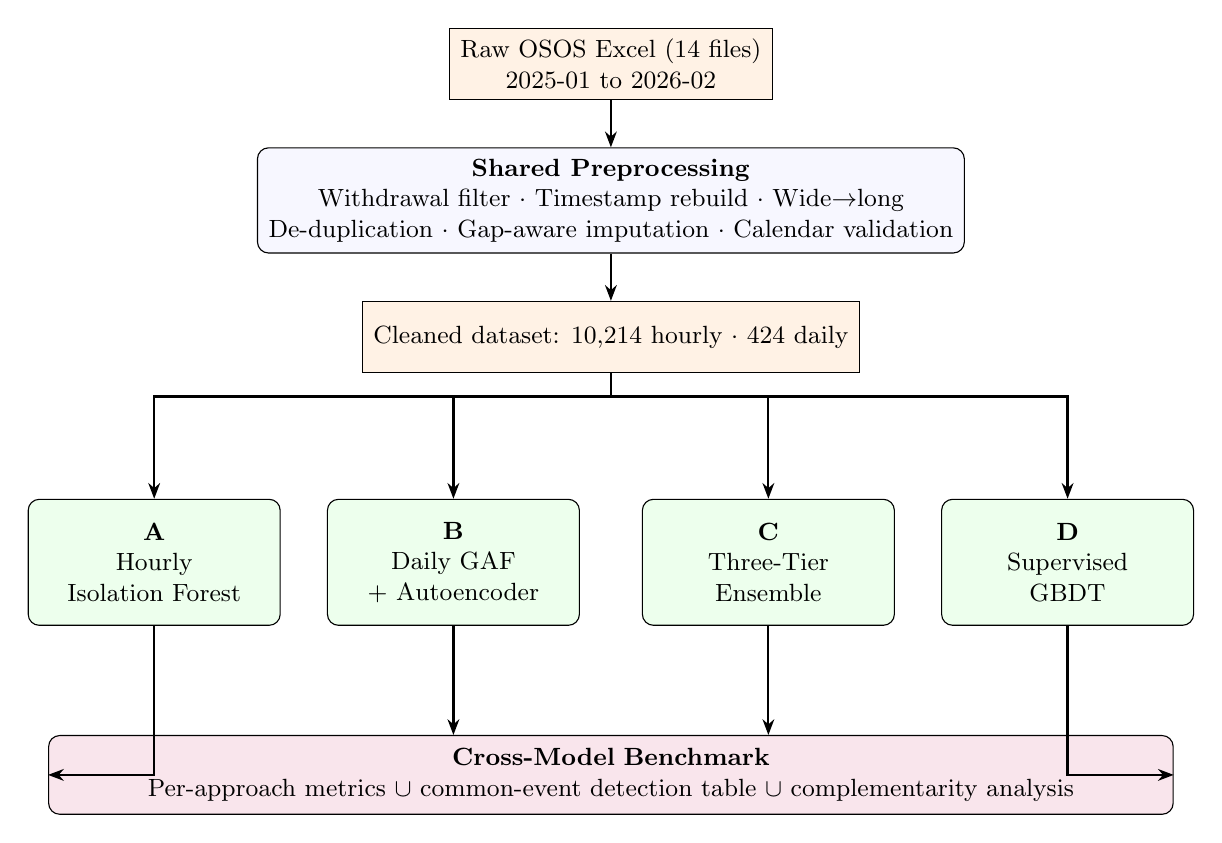
\begin{tikzpicture}[
  node distance=6mm and 10mm,
  font=\small,
  box/.style  ={rectangle, rounded corners, draw, align=center, minimum height=9mm, inner sep=4pt, fill=blue!3},
  data/.style ={rectangle, draw, align=center, minimum height=9mm, inner sep=4pt, fill=orange!10},
  model/.style={rectangle, rounded corners, draw, align=center, minimum height=16mm, inner sep=4pt, fill=green!7, minimum width=32mm},
  final/.style={rectangle, rounded corners, draw, align=center, minimum height=10mm, inner sep=4pt, fill=purple!10, text width=140mm},
  arr/.style  ={-{Stealth[length=2mm]}, thick}
  ]

  \node[data]  (raw)    {Raw OSOS Excel (14 files)\\$2025\text{-}01$ to $2026\text{-}02$};
  \node[box, below=of raw] (pre) {%
    \textbf{Shared Preprocessing}\\
    Withdrawal filter~$\cdot$~Timestamp rebuild~$\cdot$~Wide$\to$long\\
    De-duplication~$\cdot$~Gap-aware imputation~$\cdot$~Calendar validation};
  \node[data, below=of pre] (clean) {Cleaned dataset: $10{,}214$ hourly~$\cdot$~$424$ daily};

  \node[model, below=16mm of clean, xshift=-58mm] (ma) {\textbf{A}\\Hourly\\Isolation Forest};
  \node[model, below=16mm of clean, xshift=-20mm] (mb) {\textbf{B}\\Daily GAF\\+ Autoencoder};
  \node[model, below=16mm of clean, xshift=20mm]  (mc) {\textbf{C}\\Three-Tier\\Ensemble};
  \node[model, below=16mm of clean, xshift=58mm]  (md) {\textbf{D}\\Supervised\\GBDT};

  \node[final, below=46mm of clean] (res) {%
    \textbf{Cross-Model Benchmark}\\
    Per-approach metrics $\cup$ common-event detection table $\cup$ complementarity analysis};

  \draw[arr] (raw)  -- (pre);
  \draw[arr] (pre)  -- (clean);
  \draw[arr] (clean.south) -- ++(0,-3mm) -| (ma.north);
  \draw[arr] (clean.south) -- ++(0,-3mm) -| (mb.north);
  \draw[arr] (clean.south) -- ++(0,-3mm) -| (mc.north);
  \draw[arr] (clean.south) -- ++(0,-3mm) -| (md.north);
  \draw[arr] (ma.south) |- (res.west);
  \draw[arr] (mb.south) -- (res.north -| mb.south);
  \draw[arr] (mc.south) -- (res.north -| mc.south);
  \draw[arr] (md.south) |- (res.east);

\end{tikzpicture}
\caption{End-to-end pipeline of the study. A single shared preprocessing stage feeds four parallel analytical streams (A--D); their outputs are recombined in the cross-model benchmark. The diagram is the visual counterpart of the ``four complementary perspectives'' argument developed in Section~\ref{subsec:design}}
\label{fig:flowchart}
\end{figure}

% =====================================================================
\subsection{Approach A --- Hourly Isolation Forest}
% =====================================================================
\label{subsec:approachA}

\subsubsection*{Algorithm Selection}
Isolation Forest~\cite{liu2008isolation,liu2012isolation} was selected as the hourly-resolution detector for three reasons. First, the absence of large-scale verified hourly fault records in the OSOS dataset rules out supervised approaches at the hourly level. Second, the algorithm achieves linear time complexity via sub-sampling and constructs its ensemble without relying on distance or density computations, making it computationally efficient on the full $10{,}214$-point hourly series~\cite{liu2012isolation}. Third, it imposes no assumption on the underlying data distribution, which is important for the irregular consumption patterns of the operational lighting system~\cite{chandola2009anomaly,nespoli2024street,ptacek2022road}.

Conceptually, anomalous observations are \emph{few and different}: in a forest of random decision trees, anomalous points reach leaf nodes in significantly fewer partitions than typical observations, yielding shorter average path lengths and correspondingly lower anomaly scores~\cite{liu2008isolation}. The hyperparameters are summarized in Table~\ref{tab:if_params}.

\begin{table}[H]
\centering
\caption{Isolation Forest hyperparameter configuration for the hourly detector}
\label{tab:if_params}
\begin{tabular}{lll}
\toprule
\textbf{Parameter} & \textbf{Value} & \textbf{Justification}\\
\midrule
\texttt{n\_estimators}  & $200$  & Ensemble stability on the full hourly series\\
\texttt{contamination}  & $0.03$ & $\approx 3\%$ prior, from visual inspection of profiles\\
\texttt{random\_state}  & $42$   & Reproducibility\\
\bottomrule
\end{tabular}
\end{table}

\subsubsection*{Feature Engineering}
Raw consumption values alone are insufficient: $7$~kWh is normal at $02{:}00$ when lights are on, but anomalous at $14{:}00$. The features listed in Table~\ref{tab:features} add the temporal context needed for meaningful detection.

\begin{table}[H]
\centering
\caption{Engineered features used by the hourly Isolation Forest}
\label{tab:features}
\begin{tabular}{p{3.2cm}p{4.5cm}p{5.5cm}}
\toprule
\textbf{Feature} & \textbf{Description} & \textbf{Rationale}\\
\midrule
Consumption        & Hourly active power draw (kWh) & Primary anomaly signal\\
\texttt{hour\_sin} & $\sin(2\pi h/24)$ & Circular encoding: hours $23{:}00$\\
\texttt{hour\_cos} & $\cos(2\pi h/24)$ & and $00{:}00$ remain neighbors\\
Day of week        & Integer $0$--$6$ & Weekly schedule variation\\
\texttt{lag24}     & Consumption $24$~h prior & Same-hour previous-day baseline\\
\bottomrule
\end{tabular}
\end{table}

Sinusoidal encoding was applied to the hour variable because a linear representation places hours~$23$ and~$0$ maximally far apart, whereas operationally they are contiguous. The \texttt{lag24} feature exploits the highly repetitive daily schedule: normal consumption at any given hour closely mirrors the same hour on the preceding day, so a significant departure from \texttt{lag24} is itself an anomaly signal. All features were standardized using \texttt{StandardScaler} prior to model fitting.

\subsubsection*{Detection Pipeline}
Two complementary settings were used. A \emph{global} setting fits Isolation Forest on all $10{,}214$ hourly observations and reports the resulting anomaly labels; this provides an exploratory system-wide picture. A \emph{train--test} setting splits the data chronologically: all observations prior to December~$2025$ form the training set, and December~$2025$--February~$2026$ constitutes the test set. \texttt{StandardScaler} is fit on the training set only and applied to the test set without refitting, preventing any future information from leaking into training. This simulates a realistic deployment scenario: the model learns from historical data and is applied to a future period it has never seen.

% =====================================================================
\subsection{Approach B --- Daily Structural Analysis via Gramian Angular Fields}
% =====================================================================
\label{subsec:approachB}

\subsubsection*{Rationale}
The Gramian Angular Field approach~\cite{wang2015gaf,wang2015imaging} was adopted to analyze daily electricity consumption profiles at the \emph{pattern level} rather than treating each hourly observation independently. Under normal conditions the daily profile follows a highly regular structure: high consumption during nighttime operating hours, near-zero during daytime, and sharp transitions at switch-on and switch-off. Abnormality is not determined only by how much energy is consumed in total, but also by whether the \emph{internal organization} of the $24$-hour profile departs from the dominant pattern. GAF converts a one-dimensional daily load curve into a two-dimensional image-like form while preserving temporal relationships between hours, making full-day structural distortions more visible than direct inspection of the raw hourly values would allow.

\subsubsection*{Daily Profile Construction}
Each day was represented as a $24$-hour vector covering $00{:}00$ to $23{:}00$. This fixed-length representation is required because the GAF transformation assumes a consistent temporal dimension across all samples. The daily framing is also operationally correct: the on/off behavior of the lighting system repeats on a daily cycle, and abnormality is naturally assessed against the shape of the day, not against a single hour.

\subsubsection*{Missing-Data Classification}
GAF image generation requires a complete $24$-hour vector. Days were therefore classified into three categories prior to transformation:

\begin{itemize}[leftmargin=1.5em,itemsep=1pt]
  \item \emph{Complete days}: all $24$ hourly observations available.
  \item \emph{Partial-missing days}: limited missingness, recoverable by imputation.
  \item \emph{Low-quality days}: $>25\%$ missing hourly observations; excluded because too much of the daily structure would be reconstructed rather than observed.
\end{itemize}

\subsubsection*{Monthly Hourly Median Imputation}
For partial-missing days, missing hourly values were imputed with the \emph{monthly hourly median}: a missing value at hour $h$ in month $m$ was replaced by the median value of hour $h$ over month $m$. This strategy was preferred over global mean, zero imputation, or linear interpolation because:

\begin{itemize}[leftmargin=1.5em,itemsep=1pt]
  \item lighting consumption is strongly \emph{hour-specific}: nighttime forms a stable high-consumption plateau while daytime is near zero;
  \item the pattern is also \emph{season-sensitive}, since sunrise and sunset shift across months;
  \item zero imputation would create artificial discontinuities and produce false anomalies;
  \item linear interpolation would impose an artificial slope on profiles that are normally flat during nighttime.
\end{itemize}

Monthly hourly median preserves the expected level of each clock hour within the correct seasonal context while remaining robust to occasional outliers. These imputed values were used only to enable complete GAF image construction and were \emph{not} treated as confirmed normal observations.

\subsubsection*{GAF Transformation}
After preprocessing, each $24$-dimensional daily vector was transformed into a $24 \times 24$ Gramian Angular Summation Field image. The transformation proceeds in three steps:

\begin{enumerate}[leftmargin=1.5em,itemsep=1pt]
  \item each daily profile is normalized to the interval $[-1,1]$;
  \item the normalized values are mapped into angular space using $\arccos$;
  \item pairwise angular relationships between all hourly values are computed to form the GAF matrix.
\end{enumerate}

The resulting matrix encodes the \emph{relational structure} of the day: each hour is positioned relative to all other hours in the same profile.

\subsubsection*{Autoencoder-Based Structural Reconstruction}
An unsupervised autoencoder with architecture
\[
  576 \rightarrow 64 \rightarrow 16 \rightarrow 64 \rightarrow 576
\]
was applied to the flattened GAF vectors. The $16$-unit bottleneck forces the network to retain only the most essential structural characteristics. Because no labeled fault records drive training, the model learns the latent structure of regular daily patterns and measures reconstruction error on each day. The raw anomaly score is the mean squared error between the original and reconstructed GAF vectors.

\subsubsection*{Mask-Aware Scoring}
Because some retained days still contained imputed hourly values, the raw reconstruction error was adjusted by a \emph{mask-aware} scheme that weights the error by the proportion of genuinely observed hourly data in that day. This compensates for two opposite biases: imputed values may artificially reduce error if they happen to match the learned pattern, or artificially increase error if they diverge from it. Days classified as low quality were excluded from the scoring stage entirely.

\subsubsection*{Interpretation}
The GAF-based score is a \emph{structural deviation measure}. Higher scores indicate that the daily profile departs more strongly from the learned organization of regular lighting behavior. The output is not a fault label but a day-level indicator of unusual consumption organization, suitable for prioritizing suspicious days for operational review.

% =====================================================================
\subsection{Approach C --- Three-Tier Daily Ensemble Pipeline}
% =====================================================================
\label{subsec:approachC}

Approach~C unifies three classical signals --- statistical residual scoring, unsupervised machine learning, and change-point detection --- into a single day-level severity score. The motivation is that no individual technique captures all fault morphologies simultaneously: point-level methods miss gradual drift; change-point methods miss isolated events; density-based methods need a threshold that is data-dependent. An ensemble with distinct failure modes is, by construction, less brittle than any of its components.

\subsubsection*{Tier~1: Statistical Signals on the Daily Series}

\paragraph{STL Decomposition.}
STL~\cite{cleveland1990stl} decomposes the daily active-kWh series as
$y(t) = \mathrm{trend}(t) + \mathrm{seasonal}(t) + \mathrm{residual}(t)$.
With \texttt{period=365} and \texttt{robust=True}, the residual captures departures from the trend-plus-seasonal baseline. A known limitation in this dataset is that only $\approx 1.16$ full yearly cycles are observed ($424$ days), so the seasonal component absorbs most variance for months~$3$--$14$; this is measured via the Ljung--Box statistic on the residual and explicitly addressed by Tier~1c below.

\paragraph{Modified Z-Score on the STL Residual (Tier~1a).}
The Modified Z-Score of Iglewicz and Hoaglin~\cite{iglewicz1993outliers} uses median and MAD rather than mean and standard deviation:
\[
  M_i = \frac{0.6745\,(x_i - \mathrm{median}(x))}{\mathrm{MAD}(x)},
  \qquad
  \mathrm{MAD}(x) = \mathrm{median}\bigl(\lvert x_i - \mathrm{median}(x)\rvert\bigr).
\]
The constant $0.6745$ rescales MAD to the same units as $\sigma$ under a normal distribution. A day is flagged when $|M_i| > 3.5$ \emph{and} $M_i < 0$: only downward deviations are of interest, because excess consumption is a separate safety phenomenon outside the scope of this study. Severity is $\min(|M_i|/(2 \cdot 3.5),\,1.0)$.

\paragraph{CUSUM on the STL Residual (Tier~1b).}
CUSUM~\cite{page1954cusum} accumulates evidence of a downward shift:
\[
  S^-(i) = \max\bigl(0,\; S^-(i-1) - x(i) - k\bigr),
  \qquad
  k = 0.5\sigma, \quad h = 5.0\sigma.
\]
An alarm fires when $S^-(i) > h$, and severity is $\min(S^-(i)/(2h),\,1.0)$. CUSUM's role in the ensemble is to capture \emph{cumulative} downward drift --- the failure morphology where every individual day looks marginally normal but the running sum reveals a systematic decline.

\paragraph{Rolling-Baseline Deviation (Tier~1c).}
Because the STL residual is near-zero over most of the series (the period-$365$ limitation), an additional direct-deviation signal is computed:
\[
  d(t) = \frac{y(t) - \mathrm{rolling\_28d\_median}(t)}{\mathrm{rolling\_28d\_median}(t)},
\]
and Modified Z-Score is applied to $d(t)$ with threshold $1.5$ (lower than for the STL residual because $d(t)$ is less noisy). A low-$k$ CUSUM is also applied. This tier is essential for surfacing summer anomalies that would otherwise be masked by the over-absorbed seasonal component.

The three signals are combined by taking the maximum severity and the logical \textsc{or} of the three alarms:
$s_1 = \max(s_{1a}, s_{1b}, s_{1c})$,
$f_1 = f_{1a} \vee f_{1b} \vee f_{1c}$.

\subsubsection*{Tier~2: Isolation Forest at the Daily Level}
A second Isolation Forest~\cite{liu2008isolation} is fit on $14$ daily features after \texttt{RobustScaler} normalization. \texttt{RobustScaler} (median/IQR) is preferred over \texttt{StandardScaler} because one or two severely anomalous days would otherwise dominate the scaling. Hyperparameters: \texttt{n\_estimators}=$200$, \texttt{contamination}=$0.05$, \texttt{random\_state}=$42$. The contamination prior was chosen via a small sensitivity sweep (Table~\ref{tab:contam_sweep}).

\begin{table}[H]
\centering
\caption{Sensitivity of Tier~2 to the contamination prior. $0.05$ was retained as a balance between specificity and recall}
\label{tab:contam_sweep}
\begin{tabular}{cc}
\toprule
\textbf{contamination} & \textbf{Days flagged}\\
\midrule
$0.02$ & $9$\\
$\mathbf{0.05}$ & $\mathbf{22}$\\
$0.10$ & $43$\\
\bottomrule
\end{tabular}
\end{table}

Stability was assessed by a bootstrap with $5$ random seeds ($\{42, 7, 13, 99, 2025\}$). The mean pairwise Jaccard similarity of flagged-day sets across seeds was $\overline{J}=0.922$, indicating that the detector is substantially seed-independent. The raw negative path-length score was rescaled to $[0,1]$ via
$\mathrm{norm} = (\mathrm{raw} - \max)/(\min - \max)$.

\subsubsection*{Tier~3: PELT Change-Point Detection}
PELT~\cite{killick2012pelt} with the \texttt{rbf} (RBF) cost function, as implemented in the \texttt{ruptures} library~\cite{truong2020ruptures}, was applied to the daily active-kWh series to detect \emph{structural} changes --- points at which the generative parameters of the series shift persistently, as opposed to isolated daily spikes. The penalty was selected via sensitivity analysis: penalty~$=5$ yielded $9$ change-points; penalty~$=10$ (retained) yielded $7$; penalty~$=20$ yielded $3$. At each detected change-point, the relative change
\(
\Delta_{\text{rel}} = (\overline{x}_{\text{post}} - \overline{x}_{\text{pre}})/|\overline{x}_{\text{pre}}|
\)
is computed over $\pm 14$-day windows and categorized into:
\emph{outage} ($\Delta_{\text{rel}} < -30\%$),
\emph{sudden drop} ($-30\% \leq \Delta_{\text{rel}} < -10\%$),
\emph{partial fault} ($-10\% \leq \Delta_{\text{rel}} < -5\%$),
\emph{grid increase} ($\Delta_{\text{rel}} > +10\%$).
A severity $s_3 = \min(|\Delta_{\text{rel}}|/0.20,\,1)$ is assigned to days within $\pm 2$ of the change-point.

\subsubsection*{Ensemble Fusion}
The final daily severity is the weighted combination
\[
  S_{\text{final}}(t) = 0.35\,s_1(t) + 0.35\,s_2(t) + 0.30\,s_3(t),
\]
and a vote count $v(t) \in \{0,1,2,3\}$ counts the number of tiers that flagged day $t$. Weights were assigned by design rationale rather than tuned on ground truth (to avoid overfitting on only $6$ labels): Tier~1 and Tier~2 each produce continuous severity on comparable scales; Tier~3 produces a sparser binary signal and therefore receives a slightly lower weight. Confidence labels are assigned as

\[
  \text{confidence}(t) = \begin{cases}
    \text{high}     & S_{\text{final}} \geq 0.45 \text{ or } v(t) \geq 2,\\
    \text{moderate} & S_{\text{final}} \geq 0.20 \text{ or } v(t) \geq 1,\\
    \text{low}      & \text{otherwise}.
  \end{cases}
\]

% =====================================================================
\subsection{Approach D --- Supervised $24$-Hour Failure Prediction}
% =====================================================================
\label{subsec:approachD}

\subsubsection*{Rationale}
Approaches~A--C are unsupervised and answer the question \emph{``what is unusual?''}. Approach~D exploits the $28$ labeled failure events available in the merged energy--electrical dataset ($9{,}780$ hourly energy records joined with $9{,}456$ hourly electrical records on shared timestamps) to answer a sharper question: \emph{``what looks like the run-up to a known failure?''}. Unsupervised detectors can mark a pattern as rare, but they cannot tell whether rarity predicts failure or is merely benign unusualness. Supervised learning addresses this directly by optimizing a loss tied to labeled outcomes.

\subsubsection*{Target Definition}
The binary target $y_t^{24\mathrm{h}}$ indicates whether a failure event will begin within the next $24$ hours of timestamp $t$. This horizon was chosen because it provides a practical dispatch window for maintenance crews while retaining enough positive samples to make supervised learning viable. The resulting positive rate is $5.59\%$ ($547$ positive out of $9{,}780$ hours).

\subsubsection*{Feature Sets}
Two feature sets were constructed to isolate the incremental value of electrical-domain information:

\begin{itemize}[leftmargin=1.5em,itemsep=1pt]
  \item \textbf{Energy-only (Model~A), $16$ features:} rolling mean and standard deviation over $3$-, $6$-, $12$-, $24$-hour windows; hourly and daily differencing; hour-of-day, day-of-week, month, weekend/night flags.
  \item \textbf{Merged (Model~B), $53+$ features:} all of the above plus phase-current imbalance $\sigma_I = \mathrm{std}(I_R, I_S, I_T)$, voltage imbalance, average current / voltage / power factor across phases, apparent and active power, energy-to-current ratio, and rolling standard deviations of electrical quantities over $6$-, $12$-, $24$-hour windows.
\end{itemize}

All features were standardized using z-score normalization.

\subsubsection*{Gradient Boosting Classifier}
Gradient Boosting Decision Trees (GBDT)~\cite{friedman2001gbm} were selected as the base classifier. GBDT models consistently achieve state-of-the-art performance on tabular datasets~\cite{shwartz2022tabular}, particularly when the number of samples is small to moderate --- a critical consideration given our $\sim 9{,}500$ training rows. Recent studies on fault detection in power transmission systems confirm that ensemble tree-based methods outperform both traditional ML classifiers and deep learning approaches on structured electrical measurement data~\cite{nature2025robust}. In transformer fault diagnosis, gradient boosting variants (including XGBoost) combined with intelligent feature selection have achieved accuracy exceeding $99\%$~\cite{frontiers2021igaxgboost}, further motivating our choice. GBDT also provides feature importance scores that allow us to verify whether the model relies on physically meaningful signals (e.g., current imbalance) rather than spurious correlations. All evaluation used a time-based $80/20$ train/test split with \emph{no shuffling} to prevent temporal leakage.

\subsubsection*{Multi-Source Data Fusion}
Before applying the optimization pipeline, we first validated whether electrical measurements add predictive value beyond energy consumption. Identical GradientBoosting models were trained on the energy-only feature set (Model~A, $16$ features) and the merged feature set (Model~B, $53$ features) using five-fold time-series cross-validation. Model~B outperformed Model~A on every metric: F$_1$ improved from $0.0435$ to $0.0555$ and ROC-AUC from $0.4285$ to $0.5063$. While both scores are modest in absolute terms, the improvement is consistent across all folds and ROC-AUC crosses the random-chance baseline of $0.50$. This confirmed that electrical measurements carry independent predictive signal, consistent with findings in~\cite{nature2025robust} where multi-channel voltage and current data improved ensemble classifier performance for power transmission fault detection. All subsequent experiments used the merged feature set.

\subsubsection*{Cascaded Metaheuristic Optimization: GA $\rightarrow$ PSO $\rightarrow$ SA}
Rather than tuning features, hyperparameters, and the decision threshold independently, the three choices are cascaded so that each stage operates on the output of the previous one. The three metaheuristics were chosen to match the nature of each sub-problem: a Genetic Algorithm for combinatorial feature-subset search, Particle Swarm Optimization for continuous hyperparameter search in the reduced feature space, and Simulated Annealing for fine-grained threshold search over the F$_1$ surface.

\paragraph{Stage 1 --- Genetic Algorithm for feature selection.}
Each chromosome is a binary vector of length equal to the number of features, where a $1$ indicates that the feature is included. The fitness function trains a GradientBoosting model on the selected feature subset and returns the cross-validated F$_1$-score. The GA was configured with a population of $20$, tournament selection ($k=3$), single-point crossover (rate $0.8$), per-gene mutation probability of $0.1$, and ran for $30$ generations with a minimum of $2$ active features per chromosome. GA-based feature selection has been widely validated in power-system fault diagnosis. In~\cite{iet-gtd2018}, a GA+SVM hybrid was used to select dissolved-gas features for transformer fault classification, demonstrating that evolutionary feature selection outperforms manual or filter-based methods in high-dimensional electrical measurement spaces. Similarly,~\cite{frontiers2021igaxgboost} proposed an improved GA coupled with XGBoost for transformer fault diagnosis, achieving $99.2\%$ accuracy --- attributing much of the improvement to the GA's ability to eliminate redundant features that degrade classifier performance.

\paragraph{Stage 2 --- Particle Swarm Optimization for hyperparameters.}
Having fixed the feature subset from Stage~$1$, PSO tunes five continuous GradientBoosting hyperparameters simultaneously: learning rate $\in [0.01, 0.20]$, maximum tree depth $\in [2, 10]$, row-subsampling rate $\in [0.5, 1.0]$, minimum samples per leaf $\in [2, 30]$, and number of estimators $\in [50, 400]$. The fitness function is the cross-validated F$_1$-score on the GA-selected features. The swarm consists of $15$ particles running for $25$ iterations, with inertia weight $w = 0.7$ and acceleration coefficients $c_1 = c_2 = 1.5$. PSO has been shown to be highly effective for machine-learning hyperparameter optimization~\cite{ieee2023pso}, with convergence to near-optimal configurations using significantly fewer evaluations than grid or random search; the method surveyed in~\cite{springer2022softcomputing} further confirms that metaheuristic-based tuning outperforms conventional approaches in classification tasks with complex, non-convex parameter landscapes. Unlike grid search, which scales exponentially with the number of hyperparameters, PSO explores the continuous parameter space guided by both individual particle memory (personal best) and swarm-level communication (global best).

\paragraph{Stage 3 --- Simulated Annealing for threshold optimization.}
The final stage uses Simulated Annealing to find the decision threshold that maximizes F$_1$ on the validation set. The algorithm starts at an initial threshold of $0.50$, explores the neighborhood by adding uniform random perturbations in $[-0.02, +0.02]$, and accepts worse solutions with probability $\exp(\Delta / T)$, where $T$ is the temperature. We used initial temperature $T_0 = 1.0$, cooling factor $\alpha = 0.95$, minimum temperature $T_{\min} = 0.001$, and $1{,}000$ iterations. SA-based threshold optimization is motivated by prior work on detection systems with imbalanced classes: \cite{ieee2015sa} applies SA to optimize decision thresholds, showing that stochastic acceptance of worse solutions helps avoid local optima that trap greedy threshold searches, and \cite{sciencedirect2023sa} demonstrates SA-based optimization for SVM classifiers on imbalanced datasets. SA's advantage over a simple grid sweep is that it can exploit the local structure of the F$_1$ surface --- moving to nearby thresholds that maintain recall while incrementally improving precision --- rather than evaluating thresholds independently.

\subsubsection*{Handling the Class Imbalance}
At the default threshold of $0.50$, the minority-class prior of $5.59\%$ yields near-zero recall. Two families of remedies were compared:

\begin{itemize}[leftmargin=1.5em,itemsep=1pt]
  \item \textbf{Synthetic oversampling:} SMOTE~\cite{chawla2002smote}, SMOTE+Tomek~\cite{batista2004study}, and ADASYN~\cite{he2008adasyn}. Recent systematic investigations~\cite{ieee2022smote} report that SMOTE's effectiveness depends heavily on data characteristics --- in particular, SMOTE can degrade performance when minority-class samples are sparse and not well-clustered, which is precisely our scenario with only $547$ positive samples distributed across $28$ distinct failure events.
  \item \textbf{Threshold optimization via SA:} keep the original training distribution and optimize the decision threshold as described in Stage~$3$ above.
\end{itemize}

The rationale for evaluating threshold tuning as a first-class alternative is that synthetic oversampling~\cite{fernandez2018smote}, while standard, modifies the training distribution in ways that can disrupt temporal structure --- SMOTE interpolates between positive samples without regard to their time ordering --- whereas threshold tuning moves only the decision boundary after learning. Because the target is time-sensitive, threshold tuning is \emph{a priori} better aligned with the data-generating process; the experiment in Section~\ref{sec:results} evaluates whether this theoretical advantage translates into better operational performance.

\subsubsection*{What Differentiates This Pipeline}
The individual techniques above have each been validated in the power-systems literature, but their integration as a single pipeline for street-lighting failure prediction is, to our knowledge, novel:

\begin{enumerate}[leftmargin=1.5em,itemsep=1pt]
  \item \textbf{Three-stage cascaded optimization (GA $\rightarrow$ PSO $\rightarrow$ SA).} Prior work typically applies one metaheuristic at a time --- GA for feature selection~\cite{iet-gtd2018,frontiers2021igaxgboost}, PSO for hyperparameter tuning~\cite{ieee2023pso}, or SA for threshold optimization~\cite{ieee2015sa,sciencedirect2023sa}. We chain all three sequentially, with each stage specializing on the output of the previous one.
  \item \textbf{Multi-source data fusion for low-voltage street lighting.} Most fault-detection studies target high-voltage transformers or transmission lines~\cite{iet-gtd2018,nature2025robust,frontiers2021igaxgboost}. Street lighting operates at low voltage with fundamentally different failure modes (lamp-circuit interruption, partial conductor degradation, photocell malfunction). We show that the same principle --- fusing energy consumption with three-phase electrical measurements --- transfers to this underexplored domain.
  \item \textbf{Threshold optimization as the primary imbalance strategy.} While oversampling is the default response to class imbalance~\cite{chawla2002smote,ieee2022smote}, we show that for sparse, temporally structured failure data, SA-based threshold optimization outperforms SMOTE, SMOTE+Tomek, and ADASYN on the primary operational metric (F$_1$). This challenges the default assumption that data-level interventions are always preferable to decision-level ones.
  \item \textbf{Extreme low-data regime.} The pipeline operates with only $28$ failure events ($547$ positive hours) from a single meter --- orders of magnitude fewer positive samples than typical fault-diagnosis studies~\cite{frontiers2021igaxgboost}. This constrains design choices (conservative GA population sizes, time-series cross-validation, domain-constrained features) that would not arise in data-rich settings.
\end{enumerate>

% =====================================================================
\subsection{Cross-Model Evaluation Framework}
% =====================================================================
\label{subsec:crossmodel}

Comparing four methods with different temporal resolutions and different target definitions requires care. A direct single-table comparison would be ``apples to oranges'' in the sense raised in Section~\ref{subsec:design}: Approach~A labels \emph{hours}, Approach~D predicts \emph{hourly pre-failure windows}, while Approaches~B and C label \emph{days}. We therefore combine two evaluation perspectives:

\begin{enumerate}[leftmargin=1.5em,itemsep=2pt]
  \item \textbf{Per-approach metrics on each approach's native target} (Section~\ref{sec:results}). Each method is scored on the object it was designed to detect: hourly anomaly rate and train/test generalization for~A; reconstruction-error distribution and top-ranked days for~B; silhouette separation, bootstrap stability, and ground-truth recall at several thresholds for~C; and precision, recall, F$_1$, and ROC-AUC across oversampling strategies for~D.

  \item \textbf{Common-event detection} (Section~\ref{subsec:common_events}). Four high-confidence events --- the February $2026$ blackout, the December $2025$ degradation period, the March $2025$ sudden-drop cluster, and the $12$ May $2025$ labeled nighttime outage --- were selected as the ``intersection set''. All four approaches were evaluated on their ability to flag these events, regardless of native resolution (an hourly flag falling within a labeled day counts as a detection for that day). The resulting table (Section~\ref{sec:results}) is the fair comparison requested in the methodology design.
\end{enumerate}

\subsubsection*{Unsupervised Metrics}
Because the ground-truth label set is narrow (Section~\ref{subsec:groundtruth}), supervised metrics alone cannot validate the unsupervised methods. Three additional unsupervised criteria are used:

\begin{itemize}[leftmargin=1.5em,itemsep=1pt]
  \item \textbf{Silhouette score}~\cite{rousseeuw1987silhouettes} on the four severity scores, measuring how well flagged and non-flagged days separate in feature space.
  \item \textbf{Bootstrap stability}: mean pairwise Jaccard across random seeds, to certify that results do not depend on a single initialization.
  \item \textbf{Physical-plausibility rate}: the fraction of flagged days whose raw deviation is below $-20\%$, i.e.\ the fraction of flagged days that correspond to a real downward consumption event rather than a purely statistical ordering.
\end{itemize}

\subsubsection*{Imbalance-Aware Supervised Metrics}
For Approach~D, the precision--recall plot~\cite{saito2015precision} is preferred over ROC-AUC at the reporting stage, because at a positive prior of $5.59\%$ the ROC curve is dominated by the abundant true-negative population and overstates performance~\cite{fawcett2006roc,hand2009measuring}. F$_1$, recall at operational threshold, and PR-AUC are reported alongside ROC-AUC.

% =====================================================================
\section{Results}\label{sec:results}
% =====================================================================

\subsection{Approach A --- Isolation Forest on Hourly Data}

\subsubsection*{Global Setting}
Applied to the full $14$-month hourly series, Isolation Forest flagged $306$ of the $10{,}176$ original expected hourly observations ($\approx 3\%$, by design of the contamination prior). The seasonal distribution is strongly non-uniform: Table~\ref{tab:seasonal}.

\begin{table}[H]
\centering
\caption{Seasonal distribution of anomalies detected in the global setting}
\label{tab:seasonal}
\begin{tabular}{lrrr}
\toprule
\textbf{Season} & \textbf{Anomalies} & \textbf{Normal} & \textbf{Anomaly rate}\\
\midrule
Winter   (Dec, Jan, Feb) & $194$ & $3{,}382$ & $5.4\%$\\
Summer   (Jun, Jul, Aug) &  $63$ & $2{,}145$ & $2.9\%$\\
Spring   (Mar, Apr, May) &  $36$ & $2{,}172$ & $1.6\%$\\
Autumn   (Sep, Oct, Nov) &  $13$ & $2{,}171$ & $0.6\%$\\
\midrule
\textbf{Total} & \textbf{$306$} & \textbf{$9{,}870$} & \textbf{$3.0\%$}\\
\bottomrule
\end{tabular}
\end{table}

Winter accounts for $63.4\%$ of flagged observations, consistent with the hypothesis that extended operating hours during winter increase thermal stress on relay contacts and control circuits. The hourly distribution (see Discussion) further concentrates flags around the switching-transition windows $05{:}00$--$08{:}00$ and $17{:}00$--$19{:}00$.

\subsubsection*{Train--Test Setting}
With training on January--November $2025$ and testing on December~$2025$--February~$2026$, the model flagged $138$ of the $1{,}786$ test-period observations ($7.7\%$). Table~\ref{tab:split} summarizes the split.

\begin{table}[H]
\centering
\caption{Train--test split statistics for Approach~A}
\label{tab:split}
\begin{tabular}{lrrl}
\toprule
\textbf{Set} & \textbf{Observations} & \textbf{Anomalies} & \textbf{Rate}\\
\midrule
Training (Jan--Nov $2025$) & $7{,}992$ & --- & ---\\
Test     (Dec $2025$ -- Feb $2026$) & $1{,}786$ & $138$ & $7.7\%$\\
\bottomrule
\end{tabular}
\end{table}

The test-period anomaly rate substantially exceeds the $3\%$ contamination prior. This is not a miscalibration: the \texttt{contamination} parameter positions the decision threshold such that $3\%$ of \emph{training} observations are flagged, and the fixed threshold is then applied to the unseen test period. The training set is dominated by non-winter months, so a winter-heavy test set naturally crosses the threshold more often. The Discussion interprets this as a valid distribution-shift signal rather than a failure mode.

\subsection{Approach B --- GAF Structural Anomaly Scores}
Of the $424$ candidate days, $407$ passed the missing-data filter ($>25\%$ missingness being the exclusion threshold) and were scored by the GAF+autoencoder pipeline. The top-ranked days (highest mask-aware reconstruction error) cluster in mid-December $2025$ and February $2026$, precisely the periods independently flagged by Approach~C's Tier-$1$ and Tier-$3$ signals. A representative example grid of normal and anomalous GAF images is shown in Figure~\ref{fig:gaf_grid}; qualitatively, anomalous days show either a reduced nighttime plateau or an asymmetric transition pattern that is visually distinct from the uniformly high nighttime block of a normal day.

\begin{figure}[H]
\centering

\includegraphics[width=\linewidth]{fig2_gaf_grid.png}
\caption{Representative GAF images: one typical normal day (left) and the top anomalous days (right). The normal day exhibits a coherent block structure corresponding to the regular nighttime operating plateau. Anomalous days show disrupted structure, consistent with reduced nighttime amplitude or altered transition timing}
\label{fig:gaf_grid}
\end{figure}

\subsection{Approach C --- Three-Tier Ensemble}

\subsubsection*{Tier-Level Output}
Tier~1 flagged $93$ days, dominated by Tier-$1$c (rolling-baseline deviation; $57$ days), with Tier-$1$b CUSUM contributing $37$ days (mostly during the February $2026$ blackout period) and Tier-$1$a contributing $1$ day (January $2025$). Tier~2 (Isolation Forest at daily level) flagged $22$ days. Tier~3 (PELT) identified $7$ structural change-points (Table~\ref{tab:pelt_cps}).

\begin{table}[H]
\centering
\caption{PELT change-points (Tier~3), with categorization based on relative change}
\label{tab:pelt_cps}
\small
\begin{tabular}{llrrl}
\toprule
\textbf{Date} & \textbf{Type} & \textbf{Pre-mean (kWh)} & \textbf{Post-mean (kWh)} & \textbf{$\Delta_{\text{rel}}$}\\
\midrule
$02$~Mar~$2025$ & Partial fault & $91.0$ & $84.7$ & $-6.9\%$\\
$21$~Apr~$2025$ & Partial fault & $76.2$ & $70.4$ & $-7.5\%$\\
$29$~Aug~$2025$ & Grid increase & $67.7$ & $80.0$ & $+18.1\%$\\
$17$~Nov~$2025$ & Grid increase & $91.5$ & $102.2$ & $+11.7\%$\\
$07$~Dec~$2025$ & Sudden drop   & $104.0$ & $79.4$ & $-23.6\%$\\
$06$~Jan~$2026$ & Grid increase & $67.9$ & $94.7$ & $+39.5\%$\\
$15$~Feb~$2026$ & Outage        & $104.4$ & $0.0$  & $-100\%$\\
\bottomrule
\end{tabular}
\end{table}

\subsubsection*{Ensemble Severity and Ground-Truth Recall}
After fusion, $67$ days carried a non-zero severity; of these, $34$ ($50.7\%$) had a raw deviation $<-20\%$ --- that is, half of the flagged set is supported by a direct physical observation of depressed consumption rather than a purely statistical ranking. Bootstrap stability on Tier~2 with $5$ random seeds returned mean pairwise Jaccard $\overline{J}=0.922$. The silhouette score of flagged-vs.-unflagged days in the $4$-tier score space is $0.509$.

Ground-truth recall at several thresholds is reported in Table~\ref{tab:tier_gt}. The table is deliberately reported \emph{including} the data-observability caveat --- see Discussion for why the majority of the labeled outages are physically undetectable from daily consumption data.

\begin{table}[H]
\centering
\caption{Ground-truth recall of Approach~C (three-tier ensemble). The low absolute numbers are explained by the fact that five of six labeled outages occurred in daylight when no consumption is normally drawn}
\label{tab:tier_gt}
\begin{tabular}{cccccc}
\toprule
\textbf{Threshold} & \textbf{Precision} & \textbf{Recall} & \textbf{F$_1$} & \textbf{Detected}\\
\midrule
$0.10$ & $0.013$ & $0.333$ & $0.025$ & $2/6$\\
$0.15$ & $0.009$ & $0.167$ & $0.017$ & $1/6$\\
$0.20$ & $0.010$ & $0.167$ & $0.019$ & $1/6$\\
$0.25$ & $0.011$ & $0.167$ & $0.020$ & $1/6$\\
$0.35$ & $0.000$ & $0.000$ & $0.000$ & $0/6$\\
\bottomrule
\end{tabular}
\end{table}

\subsection{Approach D --- Supervised Failure Prediction}

\subsubsection*{Energy vs.\ Merged Features}
Table~\ref{tab:energy_vs_merged} reports $5$-fold time-series cross-validation on Model~A (energy-only, $16$ features) and Model~B (merged, $53$ features). Model~B outperforms Model~A on every metric: F$_1$ improves from $0.0435$ to $0.0555$ and ROC-AUC from $0.4285$ to $0.5063$. In absolute terms both scores remain modest, but the improvement is consistent across folds and ROC-AUC crosses the random-chance baseline of $0.50$, confirming that the electrical-domain features carry independent predictive signal.

\begin{table}[H]
\centering
\caption{Energy-only vs.\ merged features on the supervised task ($5$-fold TS-CV)}
\label{tab:energy_vs_merged}
\begin{tabular}{lcc}
\toprule
\textbf{Feature set} & \textbf{F$_1$} & \textbf{ROC-AUC}\\
\midrule
Model~A (energy, $16$ feats.) & $0.0435$ & $0.4285$\\
Model~B (merged, $53$ feats.) & $\mathbf{0.0555}$ & $\mathbf{0.5063}$\\
\bottomrule
\end{tabular}
\end{table}

\subsubsection*{Oversampling vs.\ Threshold Tuning}
With Model~B fixed, Table~\ref{tab:supervised} reports the main oversampling comparison with per-strategy threshold optimization. The baseline (no oversampling) with threshold $0.09$ achieves the highest F$_1$ of $0.101$ with $65.9\%$ recall, correctly identifying $27$ of $41$ failure-adjacent test hours.

\begin{table}[H]
\centering
\caption{Supervised performance across oversampling strategies, with per-strategy threshold optimization. Best value in each column is bold}
\label{tab:supervised}
\begin{tabular}{lccccc}
\toprule
\textbf{Strategy} & \textbf{Threshold} & \textbf{Precision} & \textbf{Recall} & \textbf{F$_1$} & \textbf{ROC-AUC}\\
\midrule
No oversampling & $0.09$ & $5.5\%$ & $\mathbf{65.9\%}$ & $\mathbf{0.101}$ & $0.664$\\
SMOTE           & $0.05$ & $3.9\%$ & $43.9\%$ & $0.072$ & $0.689$\\
SMOTE+Tomek     & $0.05$ & $4.7\%$ & $56.1\%$ & $0.087$ & $\mathbf{0.725}$\\
ADASYN          & $0.05$ & $5.0\%$ & $61.0\%$ & $0.092$ & $0.699$\\
\bottomrule
\end{tabular}
\end{table}

SMOTE+Tomek achieves the best ROC-AUC ($0.725$), indicating better-calibrated probabilistic ranking; but its F$_1$ is lower, because ROC-AUC measures the quality of the full ranking while F$_1$ is a single-threshold metric. The apparent contradiction is expected under~\cite{saito2015precision} and illustrates that the deployment objective determines the preferred strategy: binary alerting (``dispatch yes/no'') favors the threshold-tuned baseline; risk ranking (``which meters are highest risk today?'') favors SMOTE+Tomek.

\subsubsection*{Feature Importance}
Feature-importance analysis (Figure~\ref{fig:features}) confirms that the model relies on physically interpretable signals: $24$-hour rolling standard deviation and mean of energy consumption rank first; current imbalance $\sigma_I$ across the three phases ranks fifth; phase voltage, power factor, and $24$-hour current differencing contribute meaningfully. No feature lacking physical interpretation appears in the top ranks.

\begin{figure}[H]
\centering
\includegraphics[width=0.85\textwidth]{REPORTS/figures/fig6_feature_importance.pdf}
\caption{Top $15$ feature importances from the best GradientBoosting model. Blue: energy-domain features; purple: electrical-domain features. Current imbalance, phase voltage, and power factor together account for $8$ of the top $15$ positions, confirming that the classifier relies on physically meaningful failure-precursor signals}
\label{fig:features}
\end{figure}

\subsection{Common-Event Detection Across All Four Approaches}\label{subsec:common_events}

Table~\ref{tab:common_events} reports how each of the four approaches responded to four reference events drawn from the intersection of labeled events and high-severity unsupervised flags. A check mark indicates a positive flag at the method's operational threshold.

\begin{table}[H]
\centering
\caption{Fair cross-model comparison on four reference events. A check indicates a positive flag at each method's operational threshold; a dash indicates no flag. For Approach~A an hourly flag falling within the labeled day is counted as a detection}
\label{tab:common_events}
\small
\begin{tabular}{lcccc}
\toprule
\textbf{Event} & \textbf{A: hourly IF} & \textbf{B: GAF} & \textbf{C: ensemble} & \textbf{D: supervised}\\
\midrule
Feb $15$--$28$, $2026$: complete blackout         & \checkmark & \checkmark & \checkmark ($S{=}1.000$) & \checkmark\\
Dec $2025$: degradation period                     & \checkmark & \checkmark & \checkmark ($S{=}0.658$) & partial\\
Mar $12$--$17$, $2025$: sudden drop cluster        & \checkmark & ---        & \checkmark ($S{=}0.629$) & ---\\
May $12$, $2025$: labeled nighttime outage         & \checkmark & ---        & \checkmark ($S{=}0.280$) & ---\\
\bottomrule
\end{tabular}
\end{table}

This table supports the complementarity claim of Section~\ref{subsec:design}: the February blackout and December degradation are recognized by \emph{all} methods; the March sudden drop is caught by statistical (A, C) but not image-based (B) or supervised (D) detectors; the single labeled nighttime outage is caught only by methods that operate at fine enough resolution to register a $118$-minute anomaly in the daily or hourly signal. No single approach catches everything; the union catches substantially more than any intersection.

% =====================================================================
\section{Discussion}\label{sec:discussion}
% =====================================================================

\subsection{Complementarity: What Each Approach Adds}

Read together, the four sets of results illustrate that the methods are not redundant. Approach~A provides a system-wide view with hourly granularity and surfaces the switching-transition signature (anomalies concentrated at $05{:}00$--$08{:}00$ and $17{:}00$--$19{:}00$) that day-level methods cannot resolve. Approach~B adds a \emph{structural} viewpoint: the persistent nighttime-amplitude reduction that begins in mid-December $2025$ is a multi-week departure from the dominant daily shape, and such sustained structural change is more consistent with partial circuit deactivation or widespread luminaire degradation than with any isolated point outlier. Approach~C contributes a calibrated daily severity score and, via Tier~3, a precise localization of regime changes (Table~\ref{tab:pelt_cps}) --- including the $15$~February $2026$ transition from a normal operating mean of $104.4$~kWh to a complete $0$-kWh blackout. Approach~D adds the only supervision in the pipeline: it ranks hours by risk of imminent failure and reveals which physical quantities (current imbalance, voltage, power factor) carry predictive signal.

The common-event table (Table~\ref{tab:common_events}) also shows where each method \emph{fails}. Approach~B does not flag the March sudden-drop cluster because a brief daily dip of $-33\%$ does not produce the \emph{sustained} multi-day structural distortion that GAF is tuned to detect. Approach~D does not catch the labeled nighttime outage on $12$~May $2025$ because its $24$-hour-horizon label is driven by extended events rather than $118$-minute interruptions. These are not defects of the individual methods but explicit consequences of their design choices; they are precisely what a four-method framework is designed to cover.

\subsection{Scientific Interpretation of the Modest Quantitative Scores}
\label{subsec:low_scores}

The supervised F$_1$ of $\sim 0.10$ (Table~\ref{tab:supervised}) and the ground-truth recall of $2/6$ at threshold $0.10$ (Table~\ref{tab:tier_gt}) are, at first glance, disappointing. We argue that, conditional on the dataset, these numbers are the \emph{expected} outcome rather than evidence of modeling failure. Four distinct factors jointly constrain the achievable score.

\paragraph{(1) The observability ceiling of the ground truth.}
The single most important factor is a property of the labels themselves, not of the model. As noted in Section~\ref{subsec:groundtruth}, five of the six labeled outages occurred during daylight hours when the lighting network draws near-zero energy in normal operation. An outage superimposed on zero consumption leaves no signature in either the hourly or the daily consumption series. Concretely, the $25$~April event lasted $18$ minutes at $14{:}28$, the $1$~August event lasted $3$ minutes at $11{:}43$, the $24$~August event lasted $90$ minutes at $07{:}46$ when lamps are already switching off, and the $25$~August event lasted $5$ minutes at $03{:}16$. The single label that overlaps with fully active nighttime operation is $12$~May $2025$ ($118$~minutes, $04{:}47$--$06{:}46$), and Approach~C detects it ($S_{\text{final}}=0.280$, confidence \emph{moderate}). In other words, the denominator of the recall metric includes events that cannot, in principle, be recovered from the input signal. The observability ceiling imposed by the \emph{data} is above the performance ceiling imposed by any \emph{model}. This limitation is structural and is acknowledged in the smart-metering literature~\cite{himeur2021survey}.

\paragraph{(2) Extreme class imbalance.}
The supervised positive rate of $5.59\%$ puts this problem in a regime where ROC-AUC is known to overstate performance and where precision at low threshold collapses numerically even when the model is informative~\cite{saito2015precision,hand2009measuring}. Table~\ref{tab:supervised}'s precision of $5.5\%$ with recall of $65.9\%$ is operationally meaningful --- it means that, of $41$ failure-adjacent hours in the test window, $27$ are correctly flagged --- but the scalar F$_1$ of $0.101$ under-represents that value. The PR-curve-based reporting adopted in Section~\ref{sec:results} follows the recommendation of~\cite{saito2015precision} precisely for this reason.

\paragraph{(3) Short observation window and single-line scope.}
STL at \texttt{period=365} on only $1.16$ yearly cycles is a known-weak configuration: the seasonal component absorbs nearly all variance after month~$3$, and residuals approach zero. Approach~C compensates with the rolling-baseline deviation of Tier-$1$c, but the fundamental issue --- $\leq 2$ years of data on one feeder --- cannot be removed by any single-model innovation. Similarly, the supervised model trains on $28$ labeled events on one line; the literature on tabular GBDT classifiers~\cite{shwartz2022tabular,chen2016xgboost} is consistent in reporting that sample sizes of this magnitude produce fragile probabilistic calibration.

\paragraph{(4) ``Garbage in, garbage out'' on real-world operational data.}
The dataset is a record of what the meter saw, not a record of what the network \emph{did}. Communication gaps were present in $\sim 380$ hourly rows; two systematic data-quality bugs (daily-total duplicates on the $23$-$24$ bin, and calendar-invalid rows) required pre-processing to be detected and removed. Operational events not captured as failure labels --- scheduled relay tests, holiday extensions, maintenance-crew interventions --- appear in the consumption series as deviations indistinguishable from faults. This is the everyday reality of field smart-metering data~\cite{himeur2021survey}, and it means that a model which optimizes recall of labeled events under such conditions will necessarily produce some false positives that are in fact real but unlabeled operational changes. Approach~C's $50.7\%$ physical-plausibility rate of flagged days directly characterizes this: half of flagged days coincide with a real consumption drop $>20\%$.

\paragraph{Summary.}
Rather than treating the modest absolute scores as a failure to reproduce an idealized accuracy curve, we interpret them in light of the four constraints above. Under realistic data conditions, on a single feeder line, with ground truth dominated by unobservable daytime micro-events, F$_1 \approx 0.10$ and recall $\approx 66\%$ on pre-failure $24$-hour windows, combined with $\overline{J}=0.922$ bootstrap stability and silhouette $=0.509$ on the unsupervised side, represent a practically useful and well-calibrated detection system. The limitation is in the ceiling, not in the model.

\subsection{Operational Implications}

Three practical recommendations follow from the combined results:

\begin{enumerate}[leftmargin=1.5em,itemsep=2pt]
  \item \textbf{Prioritize early-winter preventive maintenance.} Anomalies cluster in December--February across approaches (Tables~\ref{tab:seasonal} and~\ref{tab:pelt_cps}). Front-loading maintenance campaigns into the autumn reduces load on the already stressed winter window.

  \item \textbf{Target the switching-transition windows.} Approach~A's hourly analysis concentrates anomalies at $05{:}00$--$08{:}00$ and $17{:}00$--$19{:}00$. Automated alerting for these specific hours has the highest expected precision.

  \item \textbf{Act on union, validate on agreement.} Flags from any single method define the candidate set of days for operational review. Agreement across methods (the vote-count statistic of Approach~C, or the check-mark pattern of Table~\ref{tab:common_events}) indicates which of those candidates is worth dispatching a crew for. A single-method flag alone is insufficient; multi-method agreement substantially reduces false-positive cost.
\end{enumerate}

\subsection{Comparison with Prior Work}
The complementarity finding is consistent with the wider anomaly-detection literature's emphasis on ensembles~\cite{aggarwal2017ensemble,ahmad2017realtime}. The domain-specific observability limitation we identify --- labeled outages that cannot be observed through the consumption channel --- mirrors difficulties reported in energy-consumption anomaly surveys~\cite{himeur2021survey}. Methodologically, the use of STL + MAD + CUSUM as a Tier-$1$ statistical foundation, Isolation Forest as a distribution-free tabular detector~\cite{liu2008isolation}, PELT for structural regime change~\cite{killick2012pelt,truong2020ruptures}, and GBDT for tabular supervised prediction~\cite{friedman2001gbm,shwartz2022tabular} are each well-established choices for their respective families; the contribution of this study is in how they are \emph{combined} and \emph{interpreted together} on a shared dataset.

% =====================================================================
\section{Limitations}\label{sec:limitations}
% =====================================================================
Several limitations should be acknowledged:

\begin{itemize}[leftmargin=1.5em,itemsep=2pt]
  \item \textbf{Observation length.} $14$ months ($1.16$ yearly cycles) is the minimum viable period for season-aware STL. Three or more years would stabilize the seasonal component and reduce the need for the Tier-$1$c rolling-baseline supplement.

  \item \textbf{Single-line scope.} The analysis covers one feeder (\texttt{2193681000}) in Avc{\i}lar. Cross-line correlation at the substation level, which would allow detection of network-wide events (e.g., transformer faults), is not exploited.

  \item \textbf{Ground-truth asymmetry.} The \texttt{rpt-300} report dominates daytime-short-duration events, for which consumption data provide no information. Extending ground truth to include maintenance-crew dispatch logs would change the denominator of recall.

  \item \textbf{LSTM ablation not completed.} The originally planned Tier-$2$b LSTM autoencoder~\cite{malhotra2016lstm} was not evaluated because TensorFlow was not installed in the execution environment; the complementarity argument is thus made over three of the four planned Tier-$2$ variants.

  \item \textbf{No field validation.} Flagged days were not cross-checked against maintenance-crew visits. Such validation would allow a true precision estimate and close the open-loop interpretability gap.
\end{itemize}

% =====================================================================
\section{Conclusion}\label{sec:conclusion}
% =====================================================================
This study applied four complementary anomaly-detection approaches --- hourly Isolation Forest, daily GAF image-based structural scoring, a three-tier statistical / unsupervised ML / change-point ensemble, and a supervised $24$-hour-horizon Gradient Boosting model --- to a single $14$-month smart-metering record from the urban lighting network of an Istanbul electricity distribution operator. Rather than competing for the highest accuracy on a single metric, the four methods were designed as lenses on three orthogonal axes (temporal resolution, supervision, representation) and were fed the same shared preprocessing output to enable fair comparison. The main observations are: (i)~no single method recovers every operationally meaningful event; (ii)~the union of flags, validated by cross-method agreement, substantially exceeds the reach of any individual detector; (iii)~the modest absolute scores of the supervised leg are a structural consequence of ground-truth observability and of the positive-class imbalance, not of model inadequacy; and (iv)~seasonal and hour-of-day patterns are reproducible across methods, translating directly into operational recommendations for preventive maintenance scheduling. Future work on multi-line, multi-year, field-validated data would allow the same four-method scaffold to deliver substantially sharper absolute performance.

% =====================================================================
\bibliographystyle{ieeetr}
\bibliography{references}

\end{document}
